\documentclass[a4paper, 12pt]{article}

\usepackage[top=0.5in, bottom=0.5in, left=0.9in,right=0.5in]{geometry}
\usepackage[T1]{fontenc}
\usepackage{hyperref}
\usepackage{graphicx,wrapfig}
\usepackage{enumitem}
\renewcommand{\arraystretch}{1.5}

\renewcommand{\familydefault}{\sfdefault}
\usepackage{helvet}
%\usepacakge[T1]{fontenc}

\begin{document}
%no page number
\pagestyle{empty}

\begin{wrapfigure}{r}{80pt}
	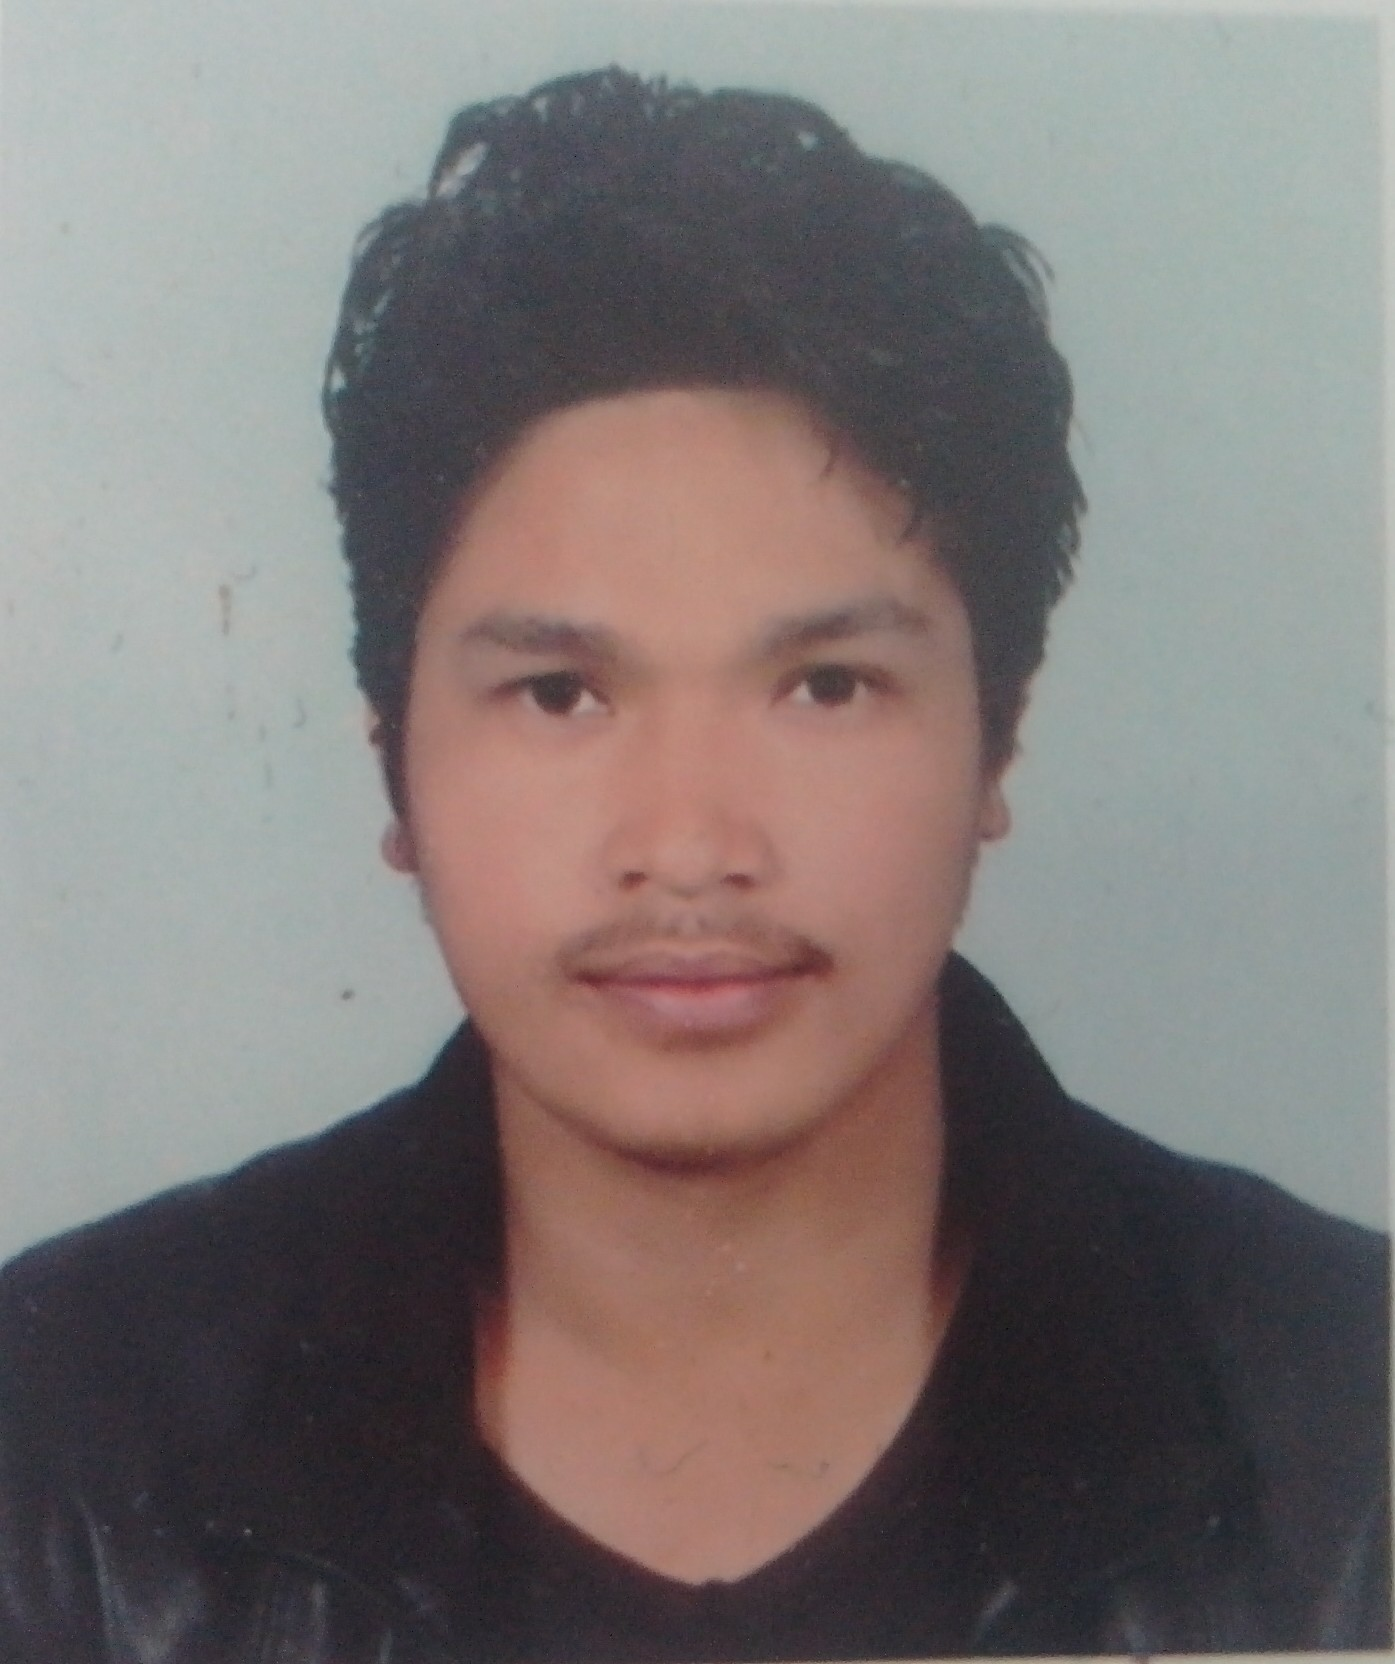
\includegraphics[height=1.5in]{k}
\end{wrapfigure}

\vspace{10mm}
{\Huge
	\textbf{Kritish Pahi} \\}
	\small{Mobile: 977 9849728755}\\
	\small{E-mail: kritishpahi@gmail.com}\\

	
\begin{wrapfigure}{c}{0in}\end{wrapfigure}
 \rule[2pt]{\textwidth}{1pt}


{ \Large \textbf{Personal Details:}\\
}
\begin{tabular}{l l}
	 \textbf{\emph{Name :}} & Kritish Pahi \\
	 \textbf{\emph{Address :}}&  Kamalbinayak -5, Bhaktapur \\
	 \textbf{\emph{Gender :}} & Male \\
	 \textbf{\emph{Marital Status :}} & Unmarried \\ 
	 \textbf{\emph{Date of birth :}} & 29 June 1995 \\ 
	 \textbf{\emph{Religion :}} & Hinduism \\ 
\end{tabular}
\vspace{8mm}

{\Large \textbf{Objective:} \\ 
}
To be an efficient Software Professional in an organization \& looking forward
to an opportunity where I can utilize my professional skills that offers 
challenges and professional growth while being resourceful, innovative 
and flexible.

\vspace{8mm}
{\Large \textbf{ Education Details: } \\
}
\begin{tabular}{l l l l}
	\textbf{Level} & \textbf{Institute} &\textbf{Year} & \textbf{Percentage} \\ \hline
	S.L.C & Prabhat English Higher Secondary School & 2011 & 88.0 \\ \hline
	H.S.E.B (Science) & Khwopa Higher Secondary School & 2013 & 82.40 \\ \hline
	B.E(Computer) & Institute of Engineering, Central Campus & 2013-Enrolling & - \\ \hline
\end{tabular}

\vspace{8mm}
{\Large \textbf{ Technical Profiles: } \\
}
\begin{tabular}{l l}
	\textbf{Languages:} & C, C++, HTML, PHP, CSS, Python, SQL \\
	\textbf{Operating System:} & Windows, Linux \\
	\textbf{Application Packages:} & MsOffice, LibreOffice, Vim, Latex \\ 
	\textbf{FrameWork: } & Bootstrap, Laravel, Django \\
	
\end{tabular}

\vspace{8mm}
{\Large \textbf{Areas of Interest:} \\
}
\vspace{-5mm}
\begin{itemize}[noitemsep]
\addtolength{\leftskip}{8mm}	
	\item Computer Networks
	\item Software Development
	\item Web Development
	\item Mobile Application Development
	\item Management

\end{itemize}

\vspace{8mm}
{\Large \textbf{Personal Skills and Strengths:}\\
}
\vspace{-5mm}
\begin{itemize}[noitemsep]
\addtolength{\leftskip}{8mm}
	\item Willingness to Learn
	\item Leadership quality
	\item Ability to be a good team player
	\item Motivating and Convincing Power
	\item Good communication skill
\end{itemize}

\vspace{8mm}

{\Large \textbf{Projects Done:} \\
}
\vspace{-5mm}
\begin{itemize}

	\item \textbf{Pacman } \emph{(2014)} \\
		\small An old, classic and popular game with Artificial Intelligence
		chasing by the ghost. Also in two player mode. C++, SDL
	\item \textbf{Multi-Security System} \emph{(2014)} \\
		\small A security system particularly designed for home application
		using laser sensor, step sensor to detect intruders. AVR 
		micro controller programming and interfacing
	\item \textbf{Gantabya} \emph{(2015)} \\
		\small A web-based as well as Android based application to recommend
		tourists about their destination based on their preference and budget
		plan. HTML, CSS, Bootstrap, PHP, MySQL, Android
	\item \textbf{Hangman} \emph{(2015)} \\
		\small Popular game among the students, guessing letters for the 
		words. Python
	\item \textbf{Alumni Database Management} \emph{(2015)}
		\small. Web based application for academic institutes to keep 
		track of Alumni of the institutes. PHP, MySQL, Laravel
	\item \textbf{EduSpace} \emph{(2016)} \\
		\small Django based website to helps students learn theories with
		their simulations and praticals. Python, Bootstrap, Django
	\item \textbf{Departmental Store Management} \emph{(2016)}
		\small Simple management of products, orders, suppliers in
		Departmental Store and mainly a website to prepare bills for 
		the goods purchased by customers. Python, Bootstrap, Django
	\item \textbf{AnswerBot} \emph{(2016)}
		\small A bot to answer to WH-question and to interact with human
		using Natual Language Processing. Python, Wiki-scraping, NER
\end{itemize}

\vspace{8mm}
{\Large \textbf{ Training and Achievements: }\\ }
%\large \textbf{Training}
\vspace{-5mm}
\begin{itemize}
	\item  Participated in Crash Courses on AVR Training (2014), Windows 
	App Developement (2014)
	\item 3rd Prize Winner in LOCUS-2014 Theme based Hardware Category 
	\emph{Multi-Security System}
	\item Ncell App camp 2015 with Top 150 ideas. \emph{Gantabya}
	\item Participation in LOCUS 2014, 2015, 2016 National Technical Fest. 
	\item Participated in Crash Course on NodeJs(2016), Mongo DB (2016) 
	\item Participated in two days \emph{Make \& Learn } Robotic Workshop
\end{itemize}



\end{document}



